\documentclass[aspectratio=169,11pt]{beamer}

\usepackage{fontspec}
\setsansfont{Latin Modern Sans}
\setmonofont{Latin Modern Mono}
\usepackage[table]{xcolor}
\usepackage{booktabs}
\usepackage{tabularx}
\usepackage{tikz}
\usetikzlibrary{arrows.meta,positioning,calc,fit,shapes.geometric}
\usepackage{pgfplots}
\pgfplotsset{compat=1.18}
\usepackage{siunitx}
\usepackage{hyperref}

\definecolor{UMLBlue}{HTML}{1F5A7A}
\definecolor{UMLTeal}{HTML}{287D7D}
\definecolor{UMLGreen}{HTML}{2E7D32}
\definecolor{UMLAmber}{HTML}{B36B00}
\definecolor{UMLRed}{HTML}{A83232}
\definecolor{UMLInk}{HTML}{182026}
\definecolor{UMLMuted}{HTML}{66717A}
\definecolor{UMLPanel}{HTML}{F3F6F8}
\definecolor{UMLGrid}{HTML}{D9E1E7}

\newcommand{\ProjectTitle}{User Mode Linux Redesign}
\newcommand{\ProjectSubtitle}{Architecture, Implementation State, and Validation Evidence}
\newcommand{\ArtifactStatus}{Historical reporting artifact}
\newcommand{\CurrentTruthNotice}{This artifact is archived at its May 2026 reporting cutoff. Current UML v2 status lives in \texttt{Documentation/virt/uml/redesign/STATUS.md} and the live sequencing inventory, not in this report or deck.}
\newcommand{\ReportDate}{May 19, 2026}
\newcommand{\CutoffCommit}{9ccbf5e7bb58}
\newcommand{\BranchName}{umlctl-deploy}
\newcommand{\KVM}{\textsf{KVM}}
\newcommand{\UML}{\textsf{UML}}
\newcommand{\Seccomp}{\texttt{seccomp}}
\newcommand{\KVMvTwo}{\texttt{kvm-v2}}
\newcommand{\umlpath}[1]{\texttt{#1}}
\newcommand{\statusdone}{\textcolor{UMLGreen}{DONE}}
\newcommand{\statusprogress}{\textcolor{UMLAmber}{IN PROGRESS}}
\newcommand{\statusblocked}{\textcolor{UMLRed}{BLOCKED}}
\newcommand{\ratio}[1]{\ensuremath{#1\times}}


\usetheme[progressbar=frametitle,numbering=fraction]{metropolis}
\metroset{block=fill}
\pgfplotsset{compat=1.18}
\setbeamertemplate{navigation symbols}{}
\setbeamercolor{normal text}{fg=UMLInk,bg=white}
\setbeamercolor{title}{fg=UMLInk}
\setbeamercolor{frametitle}{fg=white,bg=UMLBlue}
\setbeamercolor{progress bar}{fg=UMLAmber,bg=UMLGrid}
\setbeamercolor{structure}{fg=UMLBlue}
\setbeamercolor{block title}{fg=white,bg=UMLBlue}
\setbeamercolor{block body}{fg=UMLInk,bg=UMLPanel}
\setbeamerfont{frametitle}{series=\bfseries,size=\large}
\setbeamerfont{title}{series=\bfseries,size=\LARGE}

\newcommand{\pill}[2]{\colorbox{#1!14}{\textcolor{#1}{\footnotesize\textbf{#2}}}}
\newcommand{\done}{\pill{UMLGreen}{DONE}}
\newcommand{\progress}{\pill{UMLAmber}{IN PROGRESS}}
\newcommand{\planned}{\pill{UMLBlue}{PLANNED}}
\newcommand{\limit}{\pill{UMLRed}{LIMIT}}
\newcommand{\blocked}{\pill{UMLRed}{BLOCKED}}

\title{\ProjectTitle}
\subtitle{\ProjectSubtitle}
\author{Reporting cutoff: \texttt{\BranchName} @ \texttt{\CutoffCommit}}
\date{\ReportDate}

\begin{document}

\begin{frame}[plain]
\vspace*{0.35cm}
{\usebeamerfont{title}\usebeamercolor[fg]{title}\ProjectTitle\par}
\vspace{0.28cm}
{\large\ProjectSubtitle\par}
\vspace{1.0cm}
{\small Reporting cutoff:\par}
{\small\texttt{\BranchName} @ \texttt{\CutoffCommit}\par}
\vfill
{\small\ReportDate\par}
\end{frame}

\section{Goal and State}

\begin{frame}{Thesis}
\begin{columns}[T,onlytextwidth]
\column{0.53\textwidth}
\Large
\textbf{\UML{} can become a profile-driven kernel research substrate again.}

\vspace{0.7em}
\normalsize
The redesign turns one source tree into fast production, observable
research, fuzzing, sandbox, library, and time-travel artifacts.

\column{0.43\textwidth}
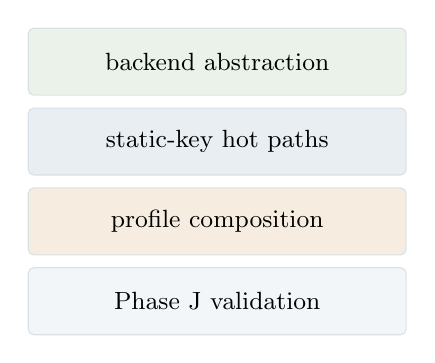
\begin{tikzpicture}[
  box/.style={draw=UMLGrid,fill=UMLPanel,rounded corners=2pt,align=center,minimum width=4.8cm,minimum height=0.85cm,font=\small},
]
\node[box,fill=UMLGreen!10] (a) {backend abstraction};
\node[box,fill=UMLBlue!10,below=0.15cm of a] (b) {static-key hot paths};
\node[box,fill=UMLAmber!12,below=0.15cm of b] (c) {profile composition};
\node[box,fill=UMLPanel,below=0.15cm of c] (d) {Phase J validation};
\end{tikzpicture}
\end{columns}
\end{frame}

\begin{frame}{Original UML, Updated}
\begin{columns}[T,onlytextwidth]
\column{0.48\textwidth}
\begin{block}{Original promise}
\begin{itemize}
  \item Linux kernel as a userspace process
  \item rootless development and debugging
  \item isolated Linux instances
  \item no machine emulation requirement
\end{itemize}
\end{block}
\column{0.48\textwidth}
\begin{block}{Modern blockers}
\begin{itemize}
  \item userspace trap cost
  \item SMP and state ownership
  \item fuzzing throughput
  \item stale profile and tooling story
\end{itemize}
\end{block}
\end{columns}
\vspace{0.45em}
\centering
\pill{UMLBlue}{RESPONSE}\quad backend abstraction + runtime gates + profile matrix + \KVMvTwo{}
\end{frame}

\begin{frame}{Goal}
\begin{columns}[T,onlytextwidth]
\column{0.50\textwidth}
\begin{block}{Build from one tree}
\begin{itemize}
  \item near-native \texttt{prod-fast}
  \item sanitizer-heavy \texttt{research}
  \item KCOV/snapshot \texttt{fuzz}
  \item minimized \texttt{sandbox}
  \item direct-call \texttt{library}
  \item deterministic \texttt{time-travel}
\end{itemize}
\end{block}
\column{0.46\textwidth}
\begin{block}{Do not build}
\begin{itemize}
  \item a Linux reimplementation
  \item a QEMU/Firecracker replacement
  \item a container runtime
  \item a from-scratch hypervisor
\end{itemize}
\end{block}
\end{columns}
\end{frame}

\begin{frame}{Current State at \ReportDate}
\small
\begin{tabularx}{\textwidth}{@{}p{0.27\textwidth}X@{}}
\toprule
Cutoff & \texttt{\CutoffCommit} on \texttt{\BranchName} \\
Functional headline & \KVMvTwo{} cleared Phases A--H, G.1/G.2, and I; Phase J is active \\
Parity & cpython-parity 21/21 under UP and SMP \\
Substrate gate & PASS=25/FAIL=3/XFAIL=3, matching seccomp \\
2h soak & \KVMvTwo{} 200/200 PASS; aggregate 397/400 PASS \\
Benchmark & Faster than seccomp on all eight hosts and all three tiers \\
\bottomrule
\end{tabularx}
\vspace{1em}
\begin{center}
\done\quad backend/gates/profile foundation
\hspace{1em}
\progress\quad Phase J validation
\hspace{1em}
\blocked\quad large upstream series until validation
\end{center}
\end{frame}

\begin{frame}{Original Versus This Branch}
\scriptsize
\begin{tabularx}{\textwidth}{@{}p{0.25\textwidth}X@{}}
\toprule
Category & Reading \\
\midrule
Inherited \UML{} and Linux & Linux-as-a-host-process, legacy ptrace,
generic kernel subsystems, existing KVM APIs, and the broad idea of
time travel are foundations, not branch-local inventions. \\
Upstream prerequisites & Seccomp-mode \UML{} and upstream SMP are
enabling context that the redesign builds on. \\
Redesigned here & Backend ops, static-key gates, profile matrix,
\KVMvTwo{} state ownership, validation ladder, and upstream sequencing. \\
Implemented here & \texttt{arch/um/backend/kvm-v2/}, profile docs and
configs, snapshot/forkserver v1, \texttt{umlctl}, launcher, gates,
soak, benchmark, and parity selftests. \\
Planned or paused & KVM-aware snapshot readiness, full record/replay,
time-machine workflow, syzkaller \texttt{vm/uml}, LTP, and upstream
\texttt{arch/um} series packaging. \\
\bottomrule
\end{tabularx}
\vspace{0.55em}
\pill{UMLBlue}{DIFF CHECK}\quad
\texttt{origin/master...HEAD} over UML paths: 688 files, 154{,}501 insertions, 823 deletions.
\end{frame}

\begin{frame}{Evidence Dashboard}
\centering
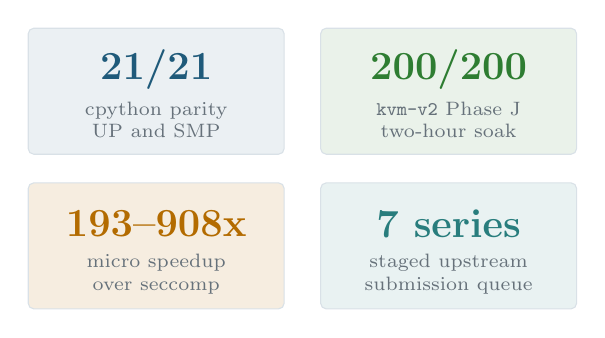
\begin{tikzpicture}[
  card/.style={draw=UMLGrid,rounded corners=2pt,minimum width=3.25cm,minimum height=1.6cm,inner sep=7pt},
  metric/.style={font=\Large\bfseries},
  label/.style={font=\scriptsize,text=UMLMuted,align=center},
]
\node[card,fill=UMLBlue!9] (a) {};
\node[metric,text=UMLBlue,yshift=0.28cm] at (a.center) {21/21};
\node[label,yshift=-0.36cm] at (a.center) {cpython parity\\UP and SMP};
\node[card,fill=UMLGreen!10,right=0.45cm of a] (b) {};
\node[metric,text=UMLGreen,yshift=0.28cm] at (b.center) {200/200};
\node[label,yshift=-0.36cm] at (b.center) {\KVMvTwo{} Phase J\\two-hour soak};
\node[card,fill=UMLAmber!12,below=0.35cm of a] (c) {};
\node[metric,text=UMLAmber,yshift=0.28cm] at (c.center) {193--908x};
\node[label,yshift=-0.36cm] at (c.center) {micro speedup\\over seccomp};
\node[card,fill=UMLTeal!10,right=0.45cm of c] (d) {};
\node[metric,text=UMLTeal,yshift=0.28cm] at (d.center) {7 series};
\node[label,yshift=-0.36cm] at (d.center) {staged upstream\\submission queue};
\end{tikzpicture}
\end{frame}

\begin{frame}{Questions to Answer}
\small
\begin{columns}[T,onlytextwidth]
\column{0.49\textwidth}
\begin{itemize}
  \item What is the revived \UML{} value proposition?
  \item Why not QEMU, Firecracker, gVisor, LKL, or containers?
  \item What architecture lets all profiles share one tree?
  \item What has landed versus what remains planned?
\end{itemize}
\column{0.49\textwidth}
\begin{itemize}
  \item Does \KVMvTwo{} preserve SMP and architectural state?
  \item Does speed survive beyond microbenchmarks?
  \item What validation bar remains before upstream?
  \item What should reviewers challenge next?
\end{itemize}
\end{columns}
\end{frame}

\section{Architecture}

\begin{frame}{Phase Map}
\centering
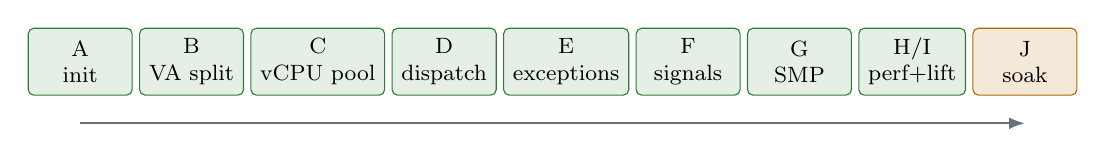
\begin{tikzpicture}[
  phase/.style={draw=UMLGrid,rounded corners=2pt,minimum width=1.32cm,minimum height=0.85cm,align=center,font=\footnotesize},
  donep/.style={draw=UMLGreen,fill=UMLGreen!12},
  progp/.style={draw=UMLAmber,fill=UMLAmber!15},
]
\node[phase,donep] (a) {A\\init};
\node[phase,donep,right=0.08cm of a] (b) {B\\VA split};
\node[phase,donep,right=0.08cm of b] (c) {C\\vCPU pool};
\node[phase,donep,right=0.08cm of c] (d) {D\\dispatch};
\node[phase,donep,right=0.08cm of d] (e) {E\\exceptions};
\node[phase,donep,right=0.08cm of e] (f) {F\\signals};
\node[phase,donep,right=0.08cm of f] (g) {G\\SMP};
\node[phase,donep,right=0.08cm of g] (h) {H/I\\perf+lift};
\node[phase,progp,right=0.08cm of h] (j) {J\\soak};
\draw[-{Latex[length=2mm]},thick,UMLMuted] ($(a.south)+(0,-0.35)$) -- ($(j.south)+(0,-0.35)$);
\end{tikzpicture}
\vspace{1em}

\begin{itemize}
  \item Old umbrella P0, Python C-extension import crashes, is functionally closed.
  \item Phase J formalizes that closure with sustained workload breadth.
\end{itemize}
\end{frame}

\begin{frame}{Three-Layer Architecture}
\centering
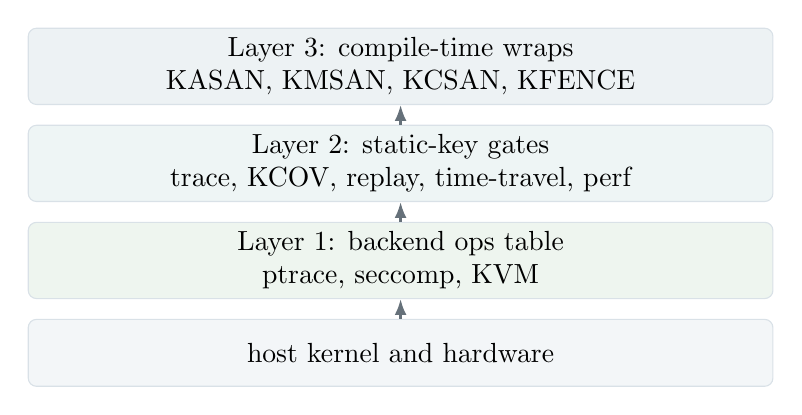
\begin{tikzpicture}[
  layer/.style={draw=UMLGrid,rounded corners=3pt,minimum width=0.78\textwidth,minimum height=0.85cm,align=center},
  arr/.style={-{Latex[length=2mm]},thick,UMLMuted},
]
\node[layer,fill=UMLBlue!8] (l3) {Layer 3: compile-time wraps\\KASAN, KMSAN, KCSAN, KFENCE};
\node[layer,fill=UMLTeal!8,below=0.25cm of l3] (l2) {Layer 2: static-key gates\\trace, KCOV, replay, time-travel, perf};
\node[layer,fill=UMLGreen!8,below=0.25cm of l2] (l1) {Layer 1: backend ops table\\ptrace, seccomp, KVM};
\node[layer,fill=UMLPanel,below=0.25cm of l1] (host) {host kernel and hardware};
\draw[arr] (host) -- (l1);
\draw[arr] (l1) -- (l2);
\draw[arr] (l2) -- (l3);
\end{tikzpicture}
\end{frame}

\begin{frame}{Layer 1: Backend Contract}
\begin{columns}[T,onlytextwidth]
\column{0.47\textwidth}
\begin{block}{Contract categories}
\begin{itemize}
  \item lifecycle and trap
  \item memory regions
  \item scheduling and IPI
  \item time
  \item debug/register access
\end{itemize}
\end{block}
\column{0.49\textwidth}
\begin{block}{Design point}
\begin{itemize}
  \item every backend implements the table
  \item single-backend builds can inline calls
  \item dynamic builds select at boot
  \item capability flags replace global backend booleans
\end{itemize}
\end{block}
\end{columns}
\end{frame}

\begin{frame}{Profiles Are Product Points}
\scriptsize
\begin{tabularx}{\textwidth}{@{}p{0.17\textwidth}p{0.19\textwidth}p{0.23\textwidth}X@{}}
\toprule
Profile & Backend & Hooks & Role \\
\midrule
prod-fast & KVM $>$ seccomp & none & near-native production \\
prod-with-hooks & KVM $>$ seccomp & compiled, off & production with emergency observability \\
research & seccomp & trace, kprobes & sanitizer/debug profile \\
fuzz & seccomp & KCOV, snapshot & syzkaller/harness fuzzing \\
fuzz-deep & seccomp & KCOV, replay & race and replay investigations \\
sandbox & seccomp-only & none compiled & minimized TCB \\
library & direct & n/a & LKL-style harnesses \\
time-travel & seccomp & deterministic time & replayable execution \\
\bottomrule
\end{tabularx}
\end{frame}

\begin{frame}{KVM v2 Model}
\centering
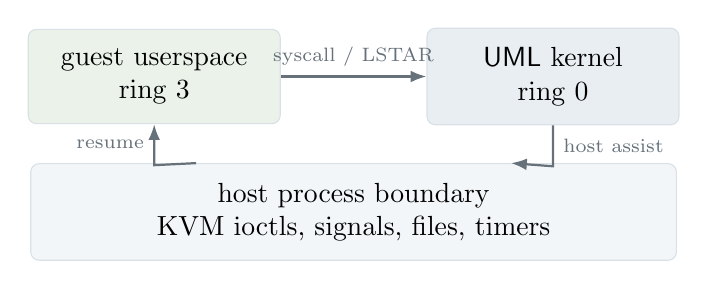
\begin{tikzpicture}[
  region/.style={draw=UMLGrid,rounded corners=3pt,align=center,inner sep=7pt,minimum height=1.0cm},
  arr/.style={-{Latex[length=2mm]},thick,UMLMuted},
  note/.style={font=\scriptsize,text=UMLMuted,align=center},
]
\node[region,fill=UMLGreen!10,minimum width=3.2cm] (user) {guest userspace\\ring 3};
\node[region,fill=UMLBlue!10,minimum width=3.2cm,right=1.85cm of user] (kernel) {\UML{} kernel\\ring 0};
\node[region,fill=UMLPanel,minimum width=8.2cm,below=1.1cm of $(user)!0.5!(kernel)$] (host) {host process boundary\\KVM ioctls, signals, files, timers};
\draw[arr] (user.east) -- node[above,note]{syscall / LSTAR} (kernel.west);
\draw[arr] (kernel.south) -- node[right,note]{host assist} ($(kernel.south)+(0,-0.52)$) -- ($(host.north)+(2.0,0)$);
\draw[arr] ($(host.north)+(-2.0,0)$) -- ($(user.south)+(0,-0.52)$) -- node[left,note]{resume} (user.south);
\end{tikzpicture}
\vspace{0.8em}

\small
This is a trap mechanism for \UML{}, not a general-purpose VMM.
\end{frame}

\begin{frame}{The Hard Part Was State Ownership}
\begin{columns}[T,onlytextwidth]
\column{0.48\textwidth}
\begin{block}{Audit inputs}
\begin{itemize}
  \item 149 state items
  \item 50+ operations
  \item ownership matrix
  \item suspect register audits
  \item runtime state trace
\end{itemize}
\end{block}
\column{0.48\textwidth}
\begin{block}{Bug classes closed}
\begin{itemize}
  \item migration while using per-CPU vCPU state
  \item EINTR mid-stub register recovery
  \item cross-task FPU/XMM leakage
  \item worker fd leak and shutdown hang
  \item AVX/XSAVE \#UD drift
\end{itemize}
\end{block}
\end{columns}
\end{frame}

\section{Validation}

\begin{frame}{Validation Ladder}
\centering
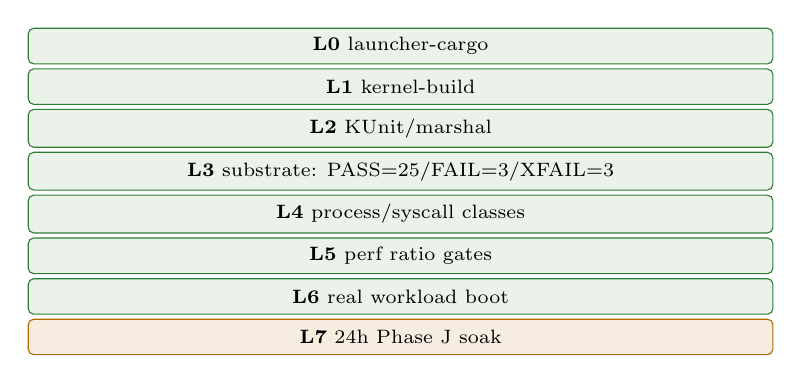
\begin{tikzpicture}[
  rung/.style={draw=UMLGrid,fill=UMLPanel,rounded corners=2pt,minimum width=0.78\textwidth,minimum height=0.45cm,align=left,inner xsep=6pt,font=\scriptsize},
  live/.style={draw=UMLGreen,fill=UMLGreen!10},
  prog/.style={draw=UMLAmber,fill=UMLAmber!12},
]
\node[rung,live] (l0) {\textbf{L0} launcher-cargo};
\node[rung,live,below=0.05cm of l0] (l1) {\textbf{L1} kernel-build};
\node[rung,live,below=0.05cm of l1] (l2) {\textbf{L2} KUnit/marshal};
\node[rung,live,below=0.05cm of l2] (l3) {\textbf{L3} substrate: PASS=25/FAIL=3/XFAIL=3};
\node[rung,live,below=0.05cm of l3] (l4) {\textbf{L4} process/syscall classes};
\node[rung,live,below=0.05cm of l4] (l5) {\textbf{L5} perf ratio gates};
\node[rung,live,below=0.05cm of l5] (l6) {\textbf{L6} real workload boot};
\node[rung,prog,below=0.05cm of l6] (l7) {\textbf{L7} 24h Phase J soak};
\end{tikzpicture}
\end{frame}

\begin{frame}{Phase J: First Sustained Run}
\small
\begin{tabular}{@{}lrrrr@{}}
\toprule
Tuple & n & pass & fail & rate \\
\midrule
\KVMvTwo{} aggregate & 200 & 200 & 0 & 100.00\% \\
seccomp aggregate & 200 & 197 & 3 & 98.50\% \\
\textbf{total} & \textbf{400} & \textbf{397} & \textbf{3} & \textbf{99.25\%} \\
\bottomrule
\end{tabular}

\vspace{1em}
\begin{itemize}
  \item 35 minutes wall before threshold-trip clean stop.
  \item Three failures were iocheck/seccomp timeout shape, not data corruption.
  \item \KVMvTwo{} passed every iteration across memcheck, iocheck, stress-ng, and tier1-pylibs.
\end{itemize}
\end{frame}

\section{Performance}

\begin{frame}{Micro Benchmark: The Gadget Changed the Cost Class}
\centering
\begin{tikzpicture}
\begin{axis}[
  width=0.9\textwidth,
  height=5.6cm,
  ybar,
  ymin=0,
  ylabel={speedup over seccomp (x)},
  symbolic x coords={s0,s1,s2,s3,s4,s5,s6,s7},
  xtick=data,
  bar width=12pt,
  fill=UMLGreen!70,
  draw=UMLGreen,
  nodes near coords,
  nodes near coords style={font=\tiny,rotate=90,anchor=west},
  grid=major,
  major grid style={draw=UMLGrid},
]
\addplot table[col sep=semicolon,x=host,y=micro]{../data/bench_speedups.csv};
\end{axis}
\end{tikzpicture}
\end{frame}

\begin{frame}{Native Baseline Context}
\small
\begin{tabularx}{\textwidth}{@{}p{0.27\textwidth}p{0.26\textwidth}X@{}}
\toprule
Path & Relative to normal & Reading \\
\midrule
Normal Linux \texttt{getpid} & 1.0x, 50 ns & Baseline used by the profile cost model. \\
\KVMvTwo{} \texttt{prod-fast} & 1.6x, 80 ns & Same order as native for gadget-covered calls. \\
\Seccomp{} profiles & 10--24x, 505--1200 ns & Expected for research, fuzz, sandbox, and time-travel. \\
ptrace fallback & 40x, 2{,}000 ns & Compatibility path, not the speed target. \\
direct library & 0.12x, 6 ns & Fast because it removes the ring split. \\
\bottomrule
\end{tabularx}
\vspace{0.7em}

\scriptsize
The cross-host benchmark still reports same-host speedup over
\Seccomp{}; this table provides user-facing native-system context.
\end{frame}

\begin{frame}{Python and Stress Tiers}
\centering
\begin{tikzpicture}
\begin{axis}[
  width=0.9\textwidth,
  height=5.6cm,
  ybar,
  ymin=0,
  ymax=10,
  ylabel={speedup over seccomp (x)},
  symbolic x coords={s0,s1,s2,s3,s4,s5,s6,s7},
  xtick=data,
  bar width=7pt,
  legend style={at={(0.5,1.06)},anchor=south,legend columns=2,draw=none,font=\footnotesize},
  grid=major,
  major grid style={draw=UMLGrid},
]
\addplot+[fill=UMLBlue!65,draw=UMLBlue] table[col sep=semicolon,x=host,y=py]{../data/bench_speedups.csv};
\addplot+[fill=UMLAmber!75,draw=UMLAmber] table[col sep=semicolon,x=host,y=stress]{../data/bench_speedups.csv};
\legend{Python,stress}
\end{axis}
\end{tikzpicture}
\end{frame}

\section{Roadmap}

\begin{frame}{Snapshot, Replay, Time Travel}
\scriptsize
\begin{tabularx}{\textwidth}{@{}p{0.27\textwidth}p{0.18\textwidth}X@{}}
\toprule
Surface & State & Reading \\
\midrule
Snapshot/forkserver v1 & \done & \texttt{um\_snapshot\_ready()},
fds 198/199, \texttt{state\_version}, launcher plumbing, and
\texttt{snapshot-smoke} are present. \\
v1 ceiling & \limit & status is hard-coded zero; no on-disk snapshot;
short non-blocking payloads only; no SMP. \\
KVM-aware readiness & \planned & Issue \#168 is unblocked but sits
behind Phase J. \\
Time-travel profile & \progress & UP/seccomp profile exists; runtime
hook gate exists; slow path is still a counter stub. \\
Record/replay/time machine & \planned & Issue \#169 covers the real
event log, replay consumer, and workflow. \\
\bottomrule
\end{tabularx}
\end{frame}

\begin{frame}{What Remains}
\begin{columns}[T,onlytextwidth]
\column{0.49\textwidth}
\begin{block}{Validation}
\begin{itemize}
  \item formal 24h Phase J
  \item Tier 2/Tier 3 templates
  \item LTP curation
  \item wider CI matrix
\end{itemize}
\end{block}
\column{0.47\textwidth}
\begin{block}{Resumed work}
\begin{itemize}
  \item KVM-aware snapshot readiness
  \item record/replay extensions
  \item syzkaller \texttt{vm/uml}
  \item optional AVX-512 Phase B
\end{itemize}
\end{block}
\end{columns}
\end{frame}

\begin{frame}{Upstream Path}
\small
\begin{tabularx}{\textwidth}{@{}r p{0.34\textwidth}p{0.2\textwidth}X@{}}
\toprule
\# & Series & Subsystem & State \\
\midrule
1 & bpf-hygiene-v1 & BPF & ready \\
2 & kmsan-arch-callback-rfc & mm/kmsan & ready \\
3 & ftrace-notrace-generic-v1 & tracing & prepared \\
4 & backend ops abstraction RFC & arch/um & to write \\
5 & static-key hot paths & arch/um & to write \\
6 & per-profile C-series & arch/um + subsystems & blocked \\
7 & KVM backend & arch/um + KVM & blocked by Phase J \\
\bottomrule
\end{tabularx}
\end{frame}

\begin{frame}{Closing Summary}
\Large
\textbf{The redesign is now an implementation with a validation frontier.}

\vspace{0.8em}
\normalsize
\begin{itemize}
  \item The architectural shape is coherent: backends, gates, profiles.
  \item \KVMvTwo{} has crossed the hardest feasibility line: real workloads, SMP, and speed.
  \item The next credible milestone is not another design memo; it is Phase J completion and an upstreamable series plan.
\end{itemize}
\end{frame}

\appendix

\begin{frame}{Backup: Detailed Speedups}
\scriptsize
\begin{tabular}{@{}llrrr@{}}
\toprule
Host & CPU & micro & Python & stress \\
\midrule
s0 & i9-12900K & 284x & 3.73x & 7.26x \\
s1 & Xeon E3-1225 v6 & 743x & 3.05x & 3.71x \\
s2 & Xeon E3-1225 v5 & 813x & 2.99x & 3.94x \\
s3 & Xeon W-2123 & 707x & 3.14x & 4.16x \\
s4 & i5-12600K & 193x & 2.99x & 8.72x \\
s5 & Ryzen 7 7840HS & 861x & 3.87x & 4.30x \\
s6 & Ryzen 7 7840HS & 908x & 4.06x & 4.32x \\
s7 & Ryzen 7 7840HS & 904x & 3.91x & 4.89x \\
\bottomrule
\end{tabular}
\end{frame}

\begin{frame}{Backup: Source Map}
\small
\begin{itemize}
  \item \texttt{00-vision.md}: goals, non-goals, stakeholders.
  \item \texttt{STATUS.md}: live state, phase ledger, blockers.
  \item \texttt{01-architecture/}: three layers, invariants, data flow.
  \item \texttt{02-workstreams/D-kvm-backend/}: KVM design, state audit, benchmarks, Phase J.
  \item \texttt{03-profiles/}: profile matrix and cost model.
  \item \texttt{tools/testing/selftests/um/}: gates, benchmarks, soak, parity.
  \item \texttt{tools/uml/uml-launcher/}: launcher and \texttt{umlctl}.
\end{itemize}
\end{frame}

\end{document}
